\documentclass[aspectratio=169,11pt]{beamer}

\usepackage[T1]{fontenc}
\usepackage{lmodern}
\usepackage{booktabs,array,xcolor,graphicx}
\usepackage{amsmath,amssymb}
\usepackage{tikz}
\usepackage{tcolorbox}
\usetikzlibrary{arrows.meta,positioning,calc,fit,backgrounds}
\tcbuselibrary{skins}

\definecolor{tplbg}{HTML}{1F4E91}      % title-slide deep blue
\definecolor{tplbg2}{HTML}{306FB0}     % title-slide gradient end
\definecolor{tpltitle}{HTML}{1B5DAA}   % frame title blue
\definecolor{tplsec}{HTML}{6E7785}     % section header grey
\definecolor{tplred}{HTML}{C0392B}     % "caveat / could help" red
\definecolor{tplgold}{HTML}{B97E08}    % "finding / exploration" gold
\definecolor{tplgreen}{HTML}{2A7D4F}   % positive number
\definecolor{tplgrey}{HTML}{A0A0A0}

\setbeamertemplate{navigation symbols}{}
\setbeamercolor{background canvas}{bg=white}
\setbeamerfont{frametitle}{size=\LARGE,series=\bfseries}
\setbeamercolor{frametitle}{fg=tpltitle,bg=white}
\setbeamertemplate{frametitle}{%
  \vspace*{0.6em}\hspace*{0.4em}%
  {\fontsize{8}{8}\selectfont\sffamily\textsc{\textcolor{tplsec}{\insertsection}}}\par%
  \vspace*{0.15em}\hspace*{0.4em}{\Large\bfseries\color{tpltitle}\insertframetitle}\par%
  \vspace*{0.4em}}
\setbeamertemplate{footline}{%
  \hfill\textcolor{tplgrey}{\tiny\insertframenumber/\inserttotalframenumber}\hspace*{1em}\vspace*{0.4em}}
\setbeamerfont{itemize/enumerate body}{size=\small}

\newtcolorbox{caveatbox}{enhanced,colback=tplred!6,colframe=tplred,boxrule=0.6pt,
  arc=2pt,left=6pt,right=6pt,top=4pt,bottom=4pt,
  borderline west={2pt}{0pt}{tplred}}
\newtcolorbox{findingbox}{enhanced,colback=tplgold!8,colframe=tplgold,boxrule=0.6pt,
  arc=2pt,left=6pt,right=6pt,top=4pt,bottom=4pt,
  borderline west={2pt}{0pt}{tplgold}}
\newcommand{\caveattag}{\textcolor{tplred}{\scriptsize\sffamily\bfseries$\Diamond$\,CAVEAT}\xspace}
\newcommand{\findingtag}{\textcolor{tplgold}{\scriptsize\sffamily\bfseries$\bigstar$\,FINDING}\xspace}
\usepackage{xspace}

% pill-style badge ("≈ 2.1 M params")
\newcommand{\pillblue}[1]{\tikz[baseline=(b.base)]{\node[fill=tpltitle,text=white,
  rounded corners=2pt,inner xsep=4pt,inner ysep=1pt,font=\scriptsize\bfseries] (b) {#1};}}
\newcommand{\pillgrey}[1]{\tikz[baseline=(b.base)]{\node[draw=tplgrey,text=tplsec,
  rounded corners=2pt,inner xsep=4pt,inner ysep=1pt,font=\scriptsize] (b) {#1};}}

% sections set the small-caps header on each frame
\AtBeginSection[]{}
\newcommand{\sectionheader}[1]{\renewcommand{\insertsection}{#1}}

\graphicspath{{figures/}{latent_viz/}{./}}

\begin{document}

{\setbeamertemplate{footline}{}
\begin{frame}[plain]
\begin{tikzpicture}[remember picture,overlay]
  \shade[left color=tplbg,right color=tplbg2] (current page.south west) rectangle (current page.north east);
\end{tikzpicture}
\vspace{1.8cm}
\begin{center}
{\color{white!85}\sffamily\fontsize{8}{8}\selectfont\textsc{Hack the World\,\,\textperiodcentered\,\,EEG track}}\\[1.4em]
{\color{white}\sffamily\fontsize{30}{34}\selectfont\bfseries EB-JEPA for Clinical EEG}\\[0.5em]
{\color{white}\sffamily\fontsize{17}{20}\selectfont A self-supervised world model on TUAB and TUEV}\\[1.9em]
{\color{white!80}\sffamily Team \textbf{vivatech-slightlyunawarefc}\,\,\textperiodcentered\,\,
  tcourtois \,\textperiodcentered\,\, yhammache \,\textperiodcentered\,\, tvasnier
  \,\,\textperiodcentered\,\, June 2026}\\[1.3em]
{\color{white!75}\sffamily\small Colour code in this deck\,---\,}%
\tikz[baseline=(b.base)]{\node[fill=tplred,text=white,rounded corners=2pt,
  inner xsep=5pt,inner ysep=2pt,font=\small\sffamily\bfseries] (b) {$\Diamond$ caveat = a limit};}\,\,%
\tikz[baseline=(b.base)]{\node[fill=tplgold,text=white,rounded corners=2pt,
  inner xsep=5pt,inner ysep=2pt,font=\small\sffamily\bfseries] (b) {$\bigstar$ finding = a result we believe};}
\end{center}
\end{frame}
}

\sectionheader{BEFORE WE START}
\begin{frame}{How to read this deck}
\begin{columns}[T,onlytextwidth]
\column{0.46\textwidth}
\textbf{What it is.}\\
A complete walk-through of our EB-JEPA submission on \textbf{TUAB} (binary
abnormal-EEG) and a transfer probe on \textbf{TUEV} (6-class events). Every number
is from our own runs --- baselines re-run from official GitHub code, EB-JEPA
trained from scratch, frozen-probed.

\vspace{0.5em}
\textbf{Two reading lenses.}
\begin{itemize}\setlength\itemsep{0pt}
  \item $\bigstar$ \textbf{Finding} (gold) --- a result that survived 3-seed re-runs / a careful caveat.
  \item $\Diamond$ \textbf{Caveat} (red) --- where we're cautious about over-claiming.
\end{itemize}

\column{0.50\textwidth}
\begin{findingbox}\findingtag One headline result\\[0.2em]
\small A 0.4\,M-param frozen self-supervised conv reaches \textbf{0.836 BAcc / 0.913 AUROC}
per-recording on TUAB --- ties supervised EEGNet, $\sim$1\,pp below a 5.8\,M foundation model,
\textbf{without seeing a single label during pretraining}.
\end{findingbox}
\vspace{0.5em}
\begin{caveatbox}\caveattag One limit\\[0.2em]
\small TUAB is close to saturation (LaBraM-Huge at 369\,M params tops out near 0.83
per-window). The interesting science lives on TUEV \& multi-task transfer.
\end{caveatbox}
\end{columns}
\end{frame}

\sectionheader{OVERVIEW \,\textperiodcentered\, THE TASK}
\begin{frame}{Clinical EEG abnormality detection on TUAB}
\begin{columns}[T,onlytextwidth]
\column{0.55\textwidth}
\begin{itemize}\setlength\itemsep{0pt}
  \item \textbf{Task:} predict \emph{normal vs.\ abnormal} from a clinical scalp EEG recording.
  \item \textbf{Why it matters:} every EEG must be reviewed by a licensed neurologist;
        labels are scarce and expensive, unlabeled data is abundant.
  \item \textbf{Benchmark: TUAB v3.0.1} (Temple Univ.\ Hospital Abnormal corpus).
  \item \textbf{Inputs:} 19\,channels, 200\,Hz, 10\,s windows (2000 samples), per-channel $z$-scored.
\end{itemize}

\vspace{0.4em}
\centering\small
\begin{tabular}{@{}lr@{}}
\toprule
& \textbf{TUAB v3.0.1} \\
\midrule
Train recordings (patients) & 2{,}717 \\
Eval  recordings (patients) & 276 \\
Class balance (eval)        & 45.7\% abnormal \\
Headline metric             & per-recording \textbf{BAcc} / \textbf{AUROC} \\
\bottomrule
\end{tabular}

\column{0.42\textwidth}
\centering
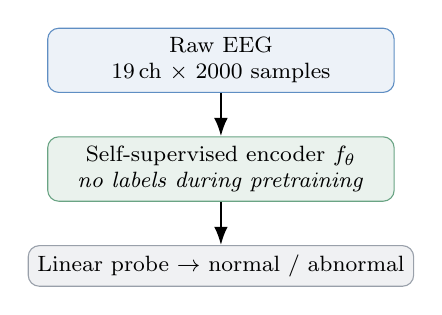
\begin{tikzpicture}[font=\footnotesize,node distance=0.55cm]
\node[draw=tpltitle!70,fill=tpltitle!8,rounded corners,minimum width=4.4cm,align=center]
  (raw) {Raw EEG\\\footnotesize 19\,ch $\times$ 2000 samples};
\node[draw=tplgreen!70,fill=tplgreen!10,rounded corners,below=of raw,minimum width=4.4cm,align=center]
  (enc) {Self-supervised encoder $f_\theta$\\\footnotesize \emph{no labels during pretraining}};
\node[draw=tplsec!70,fill=tplsec!10,rounded corners,below=of enc,minimum width=4.4cm,align=center]
  (probe) {Linear probe $\to$ normal / abnormal};
\draw[-Latex,thick] (raw) -- (enc);
\draw[-Latex,thick] (enc) -- (probe);
\end{tikzpicture}\\[0.3em]
{\scriptsize\textcolor{tplsec}{The whole pipeline. The encoder never sees a label.}}
\end{columns}
\end{frame}

\sectionheader{OVERVIEW \,\textperiodcentered\, OUR APPROACH}
\begin{frame}{EB-JEPA --- two views, one shared encoder, an anti-collapse energy}
\begin{columns}[T,onlytextwidth]
\column{0.55\textwidth}
\textbf{Energy-Based Joint-Embedding Predictive Architecture}: a single
window $x$ is corrupted twice to give views $v_1,v_2$; a shared encoder $f_\theta$
maps both, and the loss drives the latents to agree --- the encoder learns
``what is invariant to the corruption''.
\[\mathcal{L}\;=\;\underbrace{\|f_\theta(v_1)-f_\theta(v_2)\|_2^2}_{\text{invariance}}\;+\;\lambda\,\mathcal{R}(z_1,z_2)\]
\begin{itemize}\setlength\itemsep{0pt}
\item $\mathcal{R}$ is an \emph{anti-collapse} regulariser (VICReg or SIGReg).\\
      Without it, $f_\theta\equiv\mathrm{const}$ trivially minimises $\mathcal{L}$.
\item Predictor is the identity (no EMA, no stop-gradient).
\item Frozen encoder $\to$ logistic-regression probe is the headline.
\end{itemize}

\vspace{0.2em}
\pillblue{0.4 M params}\,\pillgrey{Conv1D, kernel 7, depth 4}

\column{0.42\textwidth}
\centering
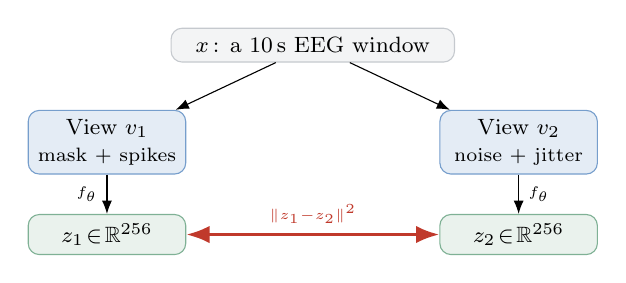
\begin{tikzpicture}[font=\footnotesize,node distance=0.35cm and 0.45cm]
\node[draw=tplsec!40,fill=tplsec!8,rounded corners,minimum width=3.6cm,align=center]
  (x) {$x$\,: a 10\,s EEG window};
\node[draw=tpltitle!60,fill=tpltitle!12,rounded corners,below left=0.6cm and -0.2cm of x,
      minimum width=2.0cm,align=center] (v1) {View $v_1$\\\scriptsize mask + spikes};
\node[draw=tpltitle!60,fill=tpltitle!12,rounded corners,below right=0.6cm and -0.2cm of x,
      minimum width=2.0cm,align=center] (v2) {View $v_2$\\\scriptsize noise + jitter};
\node[draw=tplgreen!60,fill=tplgreen!10,rounded corners,below=0.5cm of v1,
      minimum width=2.0cm,align=center] (z1) {$z_1\!\in\!\mathbb{R}^{256}$};
\node[draw=tplgreen!60,fill=tplgreen!10,rounded corners,below=0.5cm of v2,
      minimum width=2.0cm,align=center] (z2) {$z_2\!\in\!\mathbb{R}^{256}$};
\draw[-Latex] (x) -- (v1); \draw[-Latex] (x) -- (v2);
\draw[-Latex] (v1) -- (z1) node[midway,left,font=\tiny]{$f_\theta$};
\draw[-Latex] (v2) -- (z2) node[midway,right,font=\tiny]{$f_\theta$};
\draw[Latex-Latex,tplred,very thick] (z1.east) -- (z2.west)
  node[midway,above,font=\tiny\bfseries,text=tplred]{$\|z_1{-}z_2\|^2$};
\end{tikzpicture}
\end{columns}
\end{frame}

\sectionheader{OVERVIEW \,\textperiodcentered\, THE INTUITION}
\begin{frame}{Plato's Cave --- what self-supervision actually does}
\begin{columns}[T,onlytextwidth]
\column{0.55\textwidth}
Prisoners in Plato's cave see only \textbf{shadows on the wall}, not the real
objects. They learn to \emph{predict} patterns in the shadows without ever
seeing the cause.

\vspace{0.3em}
\textbf{In our setting:}
\begin{itemize}\setlength\itemsep{0pt}
  \item Cave wall = raw EEG voltages
  \item Hidden reality = underlying brain pathology
  \item SSL encoder = prisoner learning that \emph{two corrupted views of the
        same shadow are the same object}
  \item Linear probe = asking the prisoner to name what they see
\end{itemize}

\vspace{0.3em}
\textcolor{tplsec}{\footnotesize The encoder never sees a neurologist's label.
It learns structure from the signal alone --- everything downstream
(Architecture, Training, Evaluation) is about \emph{how well} it does that.}

\column{0.42\textwidth}
\centering
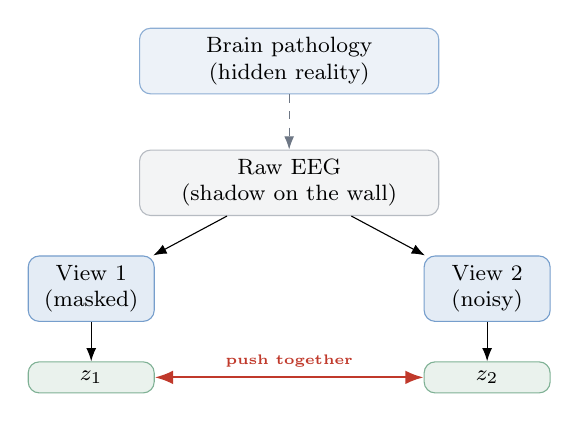
\begin{tikzpicture}[font=\footnotesize, node distance=0.5cm and 0.5cm]
  \node[draw=tpltitle!50, fill=tpltitle!8, rounded corners, minimum width=3.8cm, align=center]
    (brain) {Brain pathology\\ \footnotesize (hidden reality)};
  \node[draw=tplsec!50, fill=tplsec!8, rounded corners, below=0.7cm of brain, minimum width=3.8cm, align=center]
    (eeg) {Raw EEG\\ \footnotesize (shadow on the wall)};
  \node[draw=tpltitle!60, fill=tpltitle!12, rounded corners, below left=0.5cm and -0.2cm of eeg, minimum width=1.6cm, align=center]
    (v1) {View 1\\ \footnotesize (masked)};
  \node[draw=tpltitle!60, fill=tpltitle!12, rounded corners, below right=0.5cm and -0.2cm of eeg, minimum width=1.6cm, align=center]
    (v2) {View 2\\ \footnotesize (noisy)};
  \node[draw=tplgreen!60, fill=tplgreen!10, rounded corners, below=0.5cm of v1, minimum width=1.6cm, align=center]
    (z1) {$z_1$};
  \node[draw=tplgreen!60, fill=tplgreen!10, rounded corners, below=0.5cm of v2, minimum width=1.6cm, align=center]
    (z2) {$z_2$};
  \draw[-Latex,dashed,tplsec] (brain) -- (eeg);
  \draw[-Latex] (eeg) -- (v1); \draw[-Latex] (eeg) -- (v2);
  \draw[-Latex] (v1) -- (z1); \draw[-Latex] (v2) -- (z2);
  \draw[Latex-Latex, tplred, thick] (z1.east) -- (z2.west)
    node[midway,above,font=\tiny\bfseries,text=tplred]{push together};
\end{tikzpicture}
\end{columns}
\end{frame}

\sectionheader{DATA \,\textperiodcentered\, 1/2}
\begin{frame}{TUAB --- dataset selection \& preprocessing}
\begin{columns}[T,onlytextwidth]
\column{0.55\textwidth}
\textbf{Source.} Temple Univ.\ Hospital Abnormal EEG corpus, v3.0.1 (organisers' \texttt{TUAB\_PREPROCESSED}).

\vspace{0.3em}
\textbf{Splits (patient-disjoint).}
\begin{itemize}\setlength\itemsep{0pt}
\item train: 2{,}717 recordings (no labels seen during SSL)
\item eval:  276 recordings, $\sim$45.7\% abnormal $\to$ headline \textbf{balanced} accuracy
\item No subject overlap between train and eval.
\end{itemize}

\textbf{Pre-processing on the fly.}
\begin{itemize}\setlength\itemsep{0pt}
\item 19 channels (10--20 montage, fixed order)
\item 200\,Hz, 10\,s windows = 2000 samples, per-channel $z$-score
\item Train SSL: 20{,}000 random windows / epoch
\item Eval: 16 evenly-spaced windows / recording, probabilities mean-pooled
\end{itemize}

\column{0.42\textwidth}
\begin{caveatbox}\caveattag Preprocessing is the fairness knob\\[0.3em]
\small Every published baseline was developed with its \emph{own} preprocessing
(BIOT: 16-ch bipolar; LaBraM: learned patches; EEGNet: raw z-scored). We re-ran
\emph{their official code} on \emph{our} \texttt{TUAB\_PREPROCESSED} with a uniform
20-epoch AdamW recipe. Numbers are therefore a \textbf{uniform comparison},
not bit-exact paper reproductions.
\end{caveatbox}
\vspace{0.6em}
\begin{findingbox}\findingtag Per-window vs.\ per-recording\\[0.3em]
\small Per-rec ($\approx5$\,pp easier) is the \emph{clinical} metric;
per-window is the BIOT/LaBraM literature convention. \textbf{Mixing them
manufactures false wins}\,---\,we always report both.
\end{findingbox}
\end{columns}
\end{frame}

\sectionheader{DATA \,\textperiodcentered\, 2/2}
\begin{frame}{The two views \,---\, corruption is the lever}
\begin{columns}[T,onlytextwidth]
\column{0.55\textwidth}
\textbf{Each batch sample is loaded twice.} Two independent corruption draws
produce $v_1,v_2$ that share content (same 10\,s window) but differ in noise.

\vspace{0.3em}
\centering\small
\begin{tabular}{@{}lr@{}}
\toprule
\textbf{Augmentation} & \textbf{Strength} \\
\midrule
Gaussian noise & $\sigma=0.1$ \\
Per-channel scale-jitter & $\pm 20\%$ \\
Channel-drop & $p = 0.2$ \\
\midrule
\multicolumn{2}{l}{\textbf{Exact EB-corruption (the lever, opt-in)}} \\
\quad time-mask fraction & 20\% \\
\quad outlier-injection fraction & 20\% at $\pm 6\sigma$ \\
\quad total corrupted timepoints / view & $\approx 40\%$ \\
\bottomrule
\end{tabular}

\column{0.42\textwidth}
\begin{findingbox}\findingtag Corruption mask\,=\,single biggest lever\\[0.3em]
\small Leave-one-out ablation:
\begin{itemize}\setlength\itemsep{0pt}
\item mask: $-2.8$ pp BAcc
\item outliers: $-1.8$
\item noise: $-1.2$
\item channel-drop: $-1.0$
\item scale-jitter: $+0.2$ (dead weight)
\end{itemize}
The mask + spike-injection \emph{mimic real EEG artefacts} and force the
encoder to learn signal content, not artefact patterns.
\end{findingbox}

\vspace{0.5em}
{\small \textbf{Baseline} (``no corruption'') uses only the legacy contiguous
time-mask\,---\,this is row b in the results table.}
\end{columns}
\end{frame}

\sectionheader{ARCHITECTURE \& LOSS \,\textperiodcentered\, 1/3}
\begin{frame}{Encoders we tried}
\begin{columns}[T,onlytextwidth]
\column{0.50\textwidth}
\begin{itemize}\setlength\itemsep{0pt}
\item \textbf{1-D Conv1D} (default): 4 strided \texttt{Conv1d}, kernel 7, BN+GELU, global avg-pool.
        Scales 0.4\,M\,$\to$\,1.35\,M by widening.
\item \textbf{Transformer from scratch}: patch-embed + sinusoidal positions
        + \texttt{TransformerEncoder}, built at 1.3\,M for capacity-matched comparison.
\item \textbf{LaBraM- / BIOT- / EEGPT-style transformers}: brought up for the encoder-zoo comparison.
\end{itemize}

\vspace{0.4em}
\pillblue{Conv 0.4 M} \pillblue{Conv 1.35 M} \pillgrey{Transformer 1.3 M} \pillgrey{LaBraM-style 1.2 M} \pillgrey{BIOT-style 1.2 M} \pillgrey{EEGPT-style 0.8 M}

\vspace{0.6em}
\begin{findingbox}\findingtag Simple Conv wins at this scale\\[0.2em]
\small Capacity-matched ($\sim$1.3\,M): conv beats from-scratch Transformer by
\textbf{$-10$ pp BAcc}. The gap to SOTA transformers is \emph{pretraining
corpus + schedule}, not architecture.
\end{findingbox}

\column{0.48\textwidth}
\centering
\includegraphics[width=\linewidth]{encoder_comparison.png}\\[0.2em]
{\scriptsize\textcolor{tplsec}{Encoder ranking on TUAB
(per-rec BAcc). EEGPT collapsed under channel-drop $\times$ channel-pool conflict;
removing channel-drop alone moves it from 0.182 to 0.358 on TUEV.}}
\end{columns}
\end{frame}

\sectionheader{ARCHITECTURE \& LOSS \,\textperiodcentered\, 2/3}
\begin{frame}{The energy --- invariance + anti-collapse ($+$ spectral)}
\begin{columns}[T,onlytextwidth]
\column{0.55\textwidth}
\textbf{VICReg} (variance + covariance, the default):
\[\mathcal{L}_{\text{VIC}} = \lambda_{\rm inv}\|z_1{-}z_2\|^2 +
   \mu\,\mathcal{L}_{\rm var}(Z) + \nu\,\mathcal{L}_{\rm cov}(Z)\]
\textbullet\ $\mathcal{L}_{\rm var}$ keeps each feature's batch-std above
  margin $\gamma$ (anti-collapse).\\
\textbullet\ $\mathcal{L}_{\rm cov}$ decorrelates dimensions (info spread).

\vspace{0.3em}
\textbf{SIGReg} (LeJEPA, the principled alternative):
\[\mathcal{R}_{\rm SIG}(Z) = \tfrac{1}{P}\!\sum_p \mathcal{G}(Z\xi_p)\]
Epps--Pulley Gaussianity test on $P=256$ random projections.

\vspace{0.3em}
\textbf{Multi-scale spectral (DDSP)} on the encoder feature maps:
\[\mathcal{L}_{\rm spec}=\sum_i \|S_i{-}S_i'\|_1 + \alpha\,\|\log S_i{-}\log S_i'\|_1\]
FFT sizes $\{256,128,64,32\}$, $\alpha=1$.

\column{0.42\textwidth}
\begin{findingbox}\findingtag Spectral consistency on \emph{features}, not inputs\\[0.3em]
\small Computing the spectral term on \emph{raw} $v_1,v_2$ is constant w.r.t.\
$\theta$ ($\to$ zero gradient). Applying it to $f_\theta$'s feature maps
makes it encoder-dependent and actually backprops --- a subtle fix that
unlocks the +4\,pp lift in row 1.
\end{findingbox}

\vspace{0.4em}
\begin{caveatbox}\caveattag Stylised-facts terms are neutral\\[0.3em]
\small Adding 4 path-statistic consistency blocks ($\Delta z$, RV, ACF, sACF)
landed on the same plateau as the simpler energy (row 6 in the EB-JEPA
results table). Not a lift, not a regression.
\end{caveatbox}
\end{columns}
\end{frame}

\sectionheader{ARCHITECTURE \& LOSS \,\textperiodcentered\, 3/3}
\begin{frame}{Training dynamics}
\begin{columns}[T,onlytextwidth]
\column{0.62\textwidth}
\centering
\includegraphics[width=\linewidth]{training_curves.png}\\[0.2em]
{\scriptsize\textcolor{tplsec}{SSL loss components + validation BAcc across
20 epochs --- smooth, monotone, no collapse signal.}}

\column{0.36\textwidth}
\begin{findingbox}\findingtag No collapse\\[0.2em]
\small Per-feature std stays well above the VICReg margin $\gamma$ throughout
training; the loss decreases monotonically. No representation collapse on any
reported run.
\end{findingbox}

\vspace{0.6em}
\textbf{Observed:}
\begin{itemize}\setlength\itemsep{0pt}
\item Encoder \textbf{saturates by epoch $\sim$10}.
\item Beyond 20\,ep: no measurable gain.
\item 25\% data $\to$ $-0.8$ pp ($\Rightarrow$ not data-starved).
\end{itemize}
\end{columns}
\end{frame}

\sectionheader{TRAINING SETUP \& ITERATION}
\begin{frame}{Configuration \& fast iteration}
\begin{columns}[T,onlytextwidth]
\column{0.45\textwidth}
\centering\small
\begin{tabular}{@{}lr@{}}
\toprule
\textbf{Knob} & \textbf{Value} \\
\midrule
Optimiser     & AdamW \\
Learning rate & $10^{-3}$ (flat, no warmup) \\
Weight decay  & $10^{-6}$ \\
Batch size    & 128 \\
Epochs        & 20 \\
Windows / epoch & 20{,}000 (random) \\
\midrule
\textbf{FT recipe} & \\
\quad encoder LR mult.   & $0.1\times$ \\
\quad epochs             & 15 \\
\midrule
\textbf{Stability study} & \\
\quad Seeds                 & 0 / 1 / 2 \\
\bottomrule
\end{tabular}

\column{0.50\textwidth}
\textbf{Two-tier data strategy (proxy + full).}
\begin{enumerate}\setlength\itemsep{0pt}
\item Screen every candidate on \textbf{5\% data} / short-epoch budget.
\item Retrain only meaningful survivors on \textbf{100\% data}.
\end{enumerate}

\vspace{0.4em}
\begin{findingbox}\findingtag The proxy is predictive\\[0.2em]
\small On our conv encoder, pretraining on 25\% of recordings costs
\textbf{$<1$\,pp BAcc}\,---\,so the cheap 5\% proxy ranks runs reliably,
letting us iterate over a 5-stage campaign inside the hackathon GPU budget.
\end{findingbox}

\vspace{0.4em}
\textbf{Campaign order} (each stage keeps the best, perturbs along one axis):
capacity $\to$ augmentation $\to$ schedule $\to$ loss coefficients $\to$ data.
\end{columns}
\end{frame}

\sectionheader{INFERENCE}
\begin{frame}{The classification head --- frozen probe is the headline}
\begin{columns}[T,onlytextwidth]
\column{0.55\textwidth}
\textbf{The encoder is frozen.} We compare three classification heads:
\begin{itemize}\setlength\itemsep{0pt}
\item \textbf{Logistic probe} (headline): one linear layer on frozen features.
      Removes any probe-capacity confound. The literature-standard
      linear-evaluation protocol.
\item \textbf{Small MLP probe}: one hidden layer (256 GELU, dropout 0.3).
\item \textbf{Fine-tuned}: unfreeze the encoder, train the whole thing
      end-to-end with the linear head. Encoder LR is $0.1\times$ the head's.
\end{itemize}

\vspace{0.4em}
\textbf{Per-recording decision} (clinical):
$$\hat{y}_{\rm rec} = \mathbb{1}\!\left[\tfrac{1}{16}\sum_{w=1}^{16}\sigma(\hat{p}_w) > 0.5\right]$$
$\sigma$ is logistic; the 16 windows are evenly spaced in the recording.

\column{0.42\textwidth}
\begin{findingbox}\findingtag FT does \emph{not} beat the frozen probe\\[0.3em]
\small On our 0.4\,M conv with VICReg+corruption, fine-tuning the encoder
end-to-end gives \textbf{0.812 vs.\ 0.819 BAcc} frozen --- the SSL features
are already strong, and end-to-end training adds nothing at this scale.
\end{findingbox}

\vspace{0.4em}
\begin{caveatbox}\caveattag Cheap inference\\[0.3em]
\small One forward pass / window through 0.4\,M conv + linear read-out
$\to$ \emph{milliseconds per recording}.
\end{caveatbox}
\end{columns}
\end{frame}

\sectionheader{EVALUATION \,\textperiodcentered\, 1/3 \,\,\,\,EB-JEPA on TUAB}
\begin{frame}{Reference table --- EB-JEPA on TUAB (frozen unless noted)}
\centering\small
\begin{tabular}{@{}clccc@{}}
\toprule
\textbf{\#} & \textbf{Energy (SSL objective)} & \textbf{Encoder} & \textbf{per-rec BAcc / AUROC} & \textbf{per-win BAcc / AUROC} \\
\midrule
b & VICReg \,---\, base aug, no corruption                      & Conv 0.4M & 0.796 / 0.888 & 0.756 / --- \\
1 & \textbf{VICReg + spectral 0.1} \,(+\,corruption)               & Conv 0.4M & \textcolor{tplgreen}{\textbf{0.836 / 0.887}} & 0.765 / --- \\
2 & \textbf{SIGReg} \,(+\,corruption)                              & Conv 0.4M & 0.825 / \textcolor{tplgreen}{\textbf{0.913}} & \textcolor{tplgreen}{\textbf{0.775 / 0.856}} \\
3 & VICReg \,(+\,corruption) \,(3-seed)                            & Conv 0.4M & 0.819 $\pm$\,.004 / 0.900 $\pm$\,.006 & 0.770 / 0.848 \\
4 & VICReg \,(FT, 3-seed)                                          & Conv 0.4M & 0.812 $\pm$\,.004 / 0.908 $\pm$\,.006 & --- \\
5 & VICReg \,(multi-corpus pretraining)                            & Tr.\ 3.65M & 0.798 / 0.872 & 0.738 / --- \\
6 & VICReg + spectral + $\Delta z/\Delta z^2$/ACF/sACF \,(3-seed)  & Conv 0.4M & 0.823 $\pm$\,.007 / 0.900 $\pm$\,.010 & 0.761 / 0.841 \\
\bottomrule
\end{tabular}\\[0.3em]
{\scriptsize\textcolor{tplsec}{\texttt{reference\_table\_JEPA\_V1}\,\,\textperiodcentered\,\, $\pm$ = 3-seed std \,\,\textperiodcentered\,\, ``FT'' = fine-tuned end-to-end.}}

\vspace{0.4em}
\begin{columns}[T,onlytextwidth]
\column{0.50\textwidth}
\begin{findingbox}\findingtag Two heads tied for best\\[0.2em]
\small Row 1 (VICReg + spec) leads BAcc; row 2 (SIGReg) leads AUROC and
per-window. \emph{Both} are 0.4\,M frozen Conv.
\end{findingbox}
\column{0.46\textwidth}
\begin{caveatbox}\caveattag FT \emph{loses} to frozen on this conv\\[0.2em]
\small Row 4 $\to$ 0.812 vs.\ row 3 $\to$ 0.819. The SSL features are already
strong; end-to-end training adds nothing at 0.4\,M.
\end{caveatbox}
\end{columns}
\end{frame}

\sectionheader{EVALUATION \,\textperiodcentered\, 2/3 \,\,\,\,Robustness \& hyper-parameters}
\begin{frame}{What moves the needle --- and what doesn't}
\begin{columns}[T,onlytextwidth]
\column{0.52\textwidth}
\centering\small
\begin{tabular}{@{}clcc@{}}
\toprule
\textbf{\#} & \textbf{Test} & \textbf{per-rec BAcc} & \textbf{per-win BAcc} \\
\midrule
1  & \textbf{Tuned model} (1.35\,M)        & \textbf{0.824}            & 0.755 \\
1b & Tuned \,---\, 3-seed (mean$\pm$std)   & 0.812 $\pm$\,.021         & 0.756 $\pm$\,.001 \\
2  & Robustness \,---\, 25\% of data       & \textcolor{tplgreen}{0.816} & 0.762 \\
3  & HP \,---\, $\lambda_{\rm inv}\!=\!25$ instead of 1 & \textcolor{tplred}{0.804} & 0.730 \\
4  & Ablation \,---\, remove corruption mask           & \textcolor{tplred}{0.796} & 0.762 \\
5  & Ablation \,---\, Transformer at equal capacity    & \textcolor{tplred}{0.725} & 0.652 \\
\bottomrule
\end{tabular}\\[0.3em]
{\scriptsize\textcolor{tplsec}{\texttt{reference\_table\_robustness\_V1}}.}

\vspace{0.5em}
\includegraphics[width=\linewidth]{vicreg_fix.png}\\[0.1em]
{\scriptsize\textcolor{tplsec}{$\lambda_{\rm inv}$ sweep: monotone $1>5>10>25$.}}

\column{0.46\textwidth}
\begin{findingbox}\findingtag EEG SSL prefers \emph{weak} view-invariance\\[0.3em]
\small Full sweep:
$$\mathrm{inv}=1\ (0.824) > 5\ (0.820) > 10\ (0.814) > 25\ (0.804)$$
VICReg's vision default (25) is \textbf{2--3 pp worse} than $\mathrm{inv}=1$
on EEG ($\approx6\sigma$ across 3 seeds). Anti-collapse should \emph{dominate}
the invariance pull. The report's one novel finding.
\end{findingbox}

\vspace{0.3em}
\begin{caveatbox}\caveattag Per-rec carries $\approx\pm0.02$ seed noise\\[0.3em]
\small Row 1b: one seed dipped to 0.788. Per-window ($\pm.001$) and AUROC
($\pm.002$) are essentially deterministic. \textbf{Rank configs on per-window /
AUROC}, not single-seed per-rec.
\end{caveatbox}
\end{columns}
\end{frame}

\sectionheader{EVALUATION \,\textperiodcentered\, 3/3 \,\,\,\,Combined --- baselines vs.\ EB-JEPA}
\begin{frame}{Position vs.\ literature (per-recording-via-window)}
\begin{columns}[T,onlytextwidth]
\column{0.55\textwidth}
\centering\small
\begin{tabular}{@{}lccl@{}}
\toprule
\textbf{Model} & \textbf{BAcc} & \textbf{AUROC} & \textbf{Regime} \\
\midrule
\textbf{LaBraM-Base}            & \textbf{0.846} & \textbf{0.926} & FT (5.8\,M, foundation) \\
FFCL                            & 0.833 & 0.908 & supervised (scratch) \\
ContraWR                        & 0.830 & 0.912 & supervised (scratch) \\
ST-Transformer                  & 0.826 & 0.925 & supervised (scratch) \\
EEGNet                          & 0.824 & 0.913 & supervised (scratch) \\
\midrule
\textbf{EB-JEPA} VICReg+spec     & \textbf{0.836} & 0.887 & \textbf{frozen SSL} \\
\textbf{EB-JEPA} SIGReg          & 0.825 & \textbf{0.913} & \textbf{frozen SSL} \\
\textbf{EB-JEPA} VICReg (3-seed) & 0.812 $\pm$\,.021 & 0.898 & frozen SSL \\
\textbf{EB-JEPA} VICReg (FT)     & 0.812 $\pm$\,.004 & 0.908 & fine-tuned \\
\bottomrule
\end{tabular}

\column{0.43\textwidth}
\centering
\includegraphics[width=\linewidth]{summary_vs_baselines.png}\\[0.2em]
\begin{findingbox}\findingtag Inside the supervised cluster, no labels\\[0.2em]
\small Our 0.4\,M frozen SSL conv ties EEGNet and sits $\sim$1\,pp below
LaBraM (a 5.8\,M foundation model with external pretraining) ---
\textbf{without using any label in pretraining}.
\end{findingbox}
\end{columns}
\end{frame}

\sectionheader{TUEV \,\textperiodcentered\, FROZEN CROSS-TASK TRANSFER}
\begin{frame}{TUEV (6-class) --- the same encoder, never trained on TUEV}
\begin{columns}[T,onlytextwidth]
\column{0.55\textwidth}
\textbf{Protocol.} Freeze the TUAB-pretrained encoder; fit a class-balanced
logistic probe on TUEV event windows (5\,s @ 200\,Hz, 6 classes:
SPSW / GPED / PLED / EYEM / ARTF / BCKG).
\textbf{Zero TUEV labels during SSL.}

\vspace{0.3em}
\centering\small
\begin{tabular}{@{}lcc@{}}
\toprule
\textbf{Method} & \textbf{TUEV BAcc} & \textbf{Trained on TUEV?} \\
\midrule
ST-Transformer    & 0.339 & \textcolor{tplred}{full supervised train} \\
CNN-Transformer   & 0.410 & \textcolor{tplred}{full supervised train} \\
\midrule
\textbf{EB-JEPA} (VICReg+spec, frozen) & \textbf{0.425} & \textcolor{tplgreen}{\textbf{probe only}} \\
\textbf{EB-JEPA} (VICReg+corrupt, frozen) & 0.382 & \textcolor{tplgreen}{probe only} \\
\textbf{EB-JEPA} (SIGReg+corrupt, frozen) & 0.363 & \textcolor{tplgreen}{probe only} \\
\midrule
FFCL              & 0.455 & \textcolor{tplred}{full supervised train} \\
ContraWR          & 0.466 & \textcolor{tplred}{full supervised train} \\
BIOT (pretrained) & 0.501 & \textcolor{tplred}{full supervised train} \\
LaBraM-Huge       & 0.662 & \textcolor{tplred}{369\,M FT (cited)} \\
\bottomrule
\end{tabular}\\[0.2em]
{\scriptsize\textcolor{tplsec}{Chance = 0.167; random-encoder floor = 0.337.}}

\column{0.42\textwidth}
\begin{findingbox}\findingtag Frozen transfer beats two supervised baselines\\[0.3em]
\small A linear probe on a frozen, TUAB-only-pretrained encoder beats
CNN-Transformer and ST-Transformer that were trained end-to-end on TUEV ---
\textbf{strongest evidence that the SSL representation is genuinely general}.
\end{findingbox}

\vspace{0.4em}
\begin{caveatbox}\caveattag Not apples-to-apples to leaderboard\\[0.3em]
\small Our protocol differs from BIOT's \texttt{process.py} pipeline; LaBraM
rows are cited (different finetuning code path). Read as ``representation
transfers'', not ``new TUEV SOTA''.
\end{caveatbox}
\end{columns}
\end{frame}

\sectionheader{LATENT SPACE \,\textperiodcentered\, EB-JEPA vs.\ BIOT}
\begin{frame}{Where the signal lives --- LDA on frozen features (honest)}
\begin{columns}[T,onlytextwidth]
\column{0.48\textwidth}
\centering
{\small\textbf{EB-JEPA}\,---\,VICReg $\lambda_{\rm inv}{=}1$ + corruption}\\
{\scriptsize\textcolor{tplsec}{BAcc 0.819 \,---\, TUAB-pretrained, 0.4\,M params}}\\[0.15em]
\includegraphics[width=\linewidth]{lda_honest_tuab.png}

\column{0.48\textwidth}
\centering
{\small\textbf{BIOT (pretrained)}\,---\,SHHS+PREST 18-ch}\\
{\scriptsize\textcolor{tplsec}{BAcc 0.802 (per-win) \,---\, sleep+pathology pretraining, 1.2\,M}}\\[0.15em]
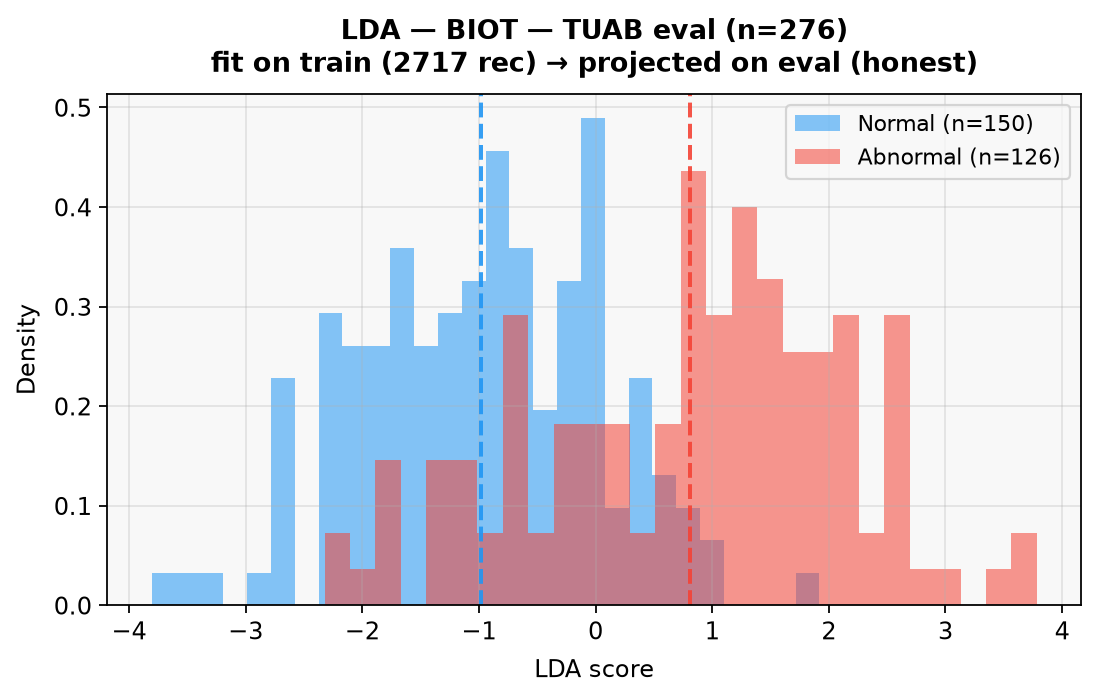
\includegraphics[width=\linewidth]{lda_honest_biot.png}
\end{columns}

\vspace{0.3em}
\begin{columns}[T,onlytextwidth]
\column{0.66\textwidth}
{\small Both LDA: \emph{fit on TUAB train} (2{,}717 recordings),
\emph{projected on TUAB eval} (276 recordings). Near-clean
separation on EB-JEPA confirms the 0.819 BAcc is real, not a probe-capacity
artefact. BIOT pretrained on sleep EEG (SHHS); domain mismatch with clinical
pathology may reduce separability.}
\column{0.32\textwidth}
\begin{findingbox}\findingtag VICReg spreads, then LDA recovers\\[0.2em]
\small Raw PCA/UMAP look mixed: VICReg spreads the signal across 256 dims
equally, so 2-D projections lose the discriminative direction. LDA, which
\emph{learns} the direction on train, recovers it.
\end{findingbox}
\end{columns}
\end{frame}

\sectionheader{LATENT SPACE \,\textperiodcentered\, 3D UMAP}
\begin{frame}{Latent space in 3D --- recovering structure 2D collapses}
\begin{columns}[T,onlytextwidth]
\column{0.62\textwidth}
\centering
\includegraphics[width=\linewidth]{latent_umap3d_window_seed0_a0.png}

\column{0.34\textwidth}
{\small\textbf{Setup.} Same encoder, window-level latents (seed 0), 3D UMAP
instead of 2D. 2{,}400 normal / 2{,}016 abnormal windows.}

\vspace{0.4em}
\begin{findingbox}\findingtag A third dimension recovers structure\\[0.2em]
\small The 2-D UMAP panel (Latent Space slide, previous) looks mixed. In 3D the
same embedding shows a two-lobe split that the 2-D projection collapses.
\end{findingbox}

\vspace{0.4em}
\begin{caveatbox}\caveattag Qualitative, not the evidence\\[0.2em]
\small Still an unsupervised projection (no labels used to fit UMAP) ---
supporting intuition for Finding 1, not the BAcc evidence itself (that's the
LDA panel, previous slide).
\end{caveatbox}
\end{columns}
\end{frame}

\sectionheader{CONCLUSION}
\begin{frame}{What we learned --- and what's next}
\begin{columns}[T,onlytextwidth]
\column{0.48\textwidth}
\textbf{\textcolor{tplgreen}{What works}}
\begin{itemize}\setlength\itemsep{0pt}
\item \textbf{Corruption augmentation} (mask + spikes): +2.3 pp BAcc, 3-seed robust.
\item \textbf{Weak invariance} $\lambda_{\rm inv}{=}1$: +2--3 pp vs.\ VICReg's vision default
  ($\approx6\sigma$), EEG-specific.
\item \textbf{SIGReg $\geq$ VICReg}: best per-window + best AUROC.
\item \textbf{TUEV transfer 0.425}: frozen, no TUEV labels, beats two supervised baselines.
\end{itemize}

\column{0.48\textwidth}
\textbf{\textcolor{tplred}{What doesn't move the needle}}
\begin{itemize}\setlength\itemsep{0pt}
\item Scaling the encoder (0.4\,M $\to$ 1.35\,M): same plateau $\Rightarrow$ capacity is not the limit.
\item 4$\times$ more pretraining data (saturates).
\item Spectral / stylised-facts terms beyond row 1's spec 0.1.
\item EEGPT-style channel-pool transformer (collapsed under channel-drop).
\end{itemize}
\end{columns}

\vspace{0.6em}
\begin{columns}[T,onlytextwidth]
\column{0.50\textwidth}
\begin{findingbox}\findingtag Open lead\\[0.2em]
\small Confirm the inv$\in\{1,5,10,25\}$ sweep $\times$ VICReg/SIGReg
$\times$ multi-seed --- ``weak invariance helps EEG SSL'' is genuinely novel.
\end{findingbox}

\column{0.46\textwidth}
\begin{caveatbox}\caveattag TUAB is near-saturated\\[0.2em]
\small Even LaBraM-Huge (369\,M) tops out near 0.83 per-window. \textbf{Pivot to
TUEV / TUSZ} where there is real headroom and SSL value shows.
\end{caveatbox}
\end{columns}
\end{frame}

{\setbeamertemplate{footline}{}
\begin{frame}[plain]
\begin{tikzpicture}[remember picture,overlay]
  \shade[left color=tplbg,right color=tplbg2] (current page.south west) rectangle (current page.north east);
\end{tikzpicture}
\vspace{2.4cm}
\begin{center}
{\color{white}\sffamily\fontsize{36}{40}\selectfont\bfseries Thank you}\\[0.7em]
{\color{white!85}\sffamily\large \emph{EB-JEPA for Clinical EEG \,---\, a first run}}\\[1.4em]
{\color{white!70}\sffamily Team \textbf{vivatech-slightlyunawarefc} \,---\, questions welcome}
\end{center}
\end{frame}
}

\end{document}
